\section{Actor Critic}
So far, we’ve explored two methods for deriving optimal policies. The first approach involves 
value-based methods, such as dynamic programming and Q-learning, where we focus on learning 
value functions (V-, Q- or Advantage-Function) and then use them to derive the policy.
The second approach is through policy gradient methods, where we directly learn the policy 
without the need for an explicit value function. Actor-Critic methods combine both of these approaches.
The critic learns a value function, while the actor learns the policy. Instead of directly using the 
critic or the actor to derive the policy, the critic's value estimates are used to guide the actor, providing 
direction for updating the policy gradient.
\begin{figure}[H]
    \centering
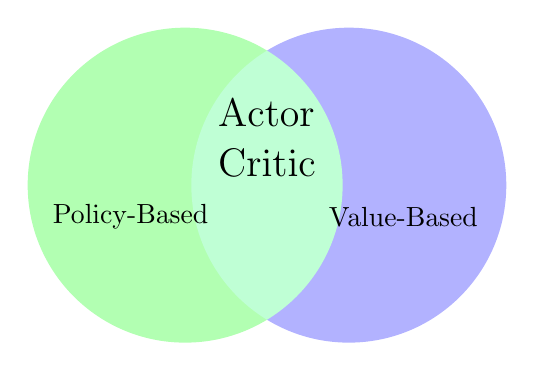
\begin{tikzpicture}
  \begin{scope}[blend group = soft light]
    \fill[green!30!white] (210:1.2) circle (2);
    \fill[blue!30!white]  (330:1.2) circle (2);
  \end{scope}
  \node at ( 210:2)   {Policy-Based};
  \node at ( 330:2)   {Value-Based};
  \node [font=\Large,align=left] {Actor\\ Critic};
\end{tikzpicture}
    \caption{Illustrating the relationship between  Actor-Critic, policy-based and value-based methods}
    \label{fig:actor_critics_venn}
\end{figure}
The most general actor-critic algorithm would look something like this:
\begin{algorithm}[H]
  \large
    \caption{One-Step Actor Critic}\label{general_actor_critic}
    \begin{algorithmic}
        \STATE Init. $s,\theta,w$
        \FOR{$t=0,1,\dots,T$}
        \STATE sample $a_t \sim \pi_{\theta}(s_t)$
        \STATE sample $s_{t+1} \sim P(s_{t+1}|s_t,a_t)$ and  $r_{t+1} \sim R(s_t,a_t)$
        %\STATE $w \gets w + \beta \delta_t\nabla_w V_w(s_t)$
        \STATE Update $V^\pi_w$
        \STATE $A^\pi(s_t,a_t) = r_{t+1} + \gamma V^\pi_{w}(s_{t+1})- V^\pi_{w}(s_t)$
        \STATE $\nabla_\theta J(\theta) \approx \nabla_\theta \log{\pi(a_t|s_t)A^\pi(s_t,a_t)}$
        \STATE $\theta \gets \theta + \alpha \nabla_\theta J(\theta) $
        \ENDFOR
    \end{algorithmic}
\end{algorithm}
There are multiple variants of the actor-critics method which will be looking at in the following.
